% % 主文档,包含了 SZU Master Thesis LaTex 全篇的主要架构。

% % 载入模板类
% \documentclass{szuthesis}  % 默认形式
% \documentclass[print]{szuthesis}  % 打印预览版本,可自动生成额外的空白页用于打印
% \documentclass[fontset=windows|adobe|mac|ubuntu]{szuthesis}  % 选择字库
\documentclass[fontset=windows]{szuthesis}

% % 载入配置信息,包含论文封面信息、必要的package
% % config.tex,传入一些参数到szuthesis.cls用来生成封面信息,并定义了一些可选的宏包(如数学公式字体、代码片段、超链接等)。

\classid{}  % 分类号
\udc{}
\confidential{}  % 密级

% % 中文题目,包含两个参数
\title{中文题目}{}  % 单行题目,第二个参数为空
% \title{论文题目第一行}{第二行}  % 多行题目
% % 英文题目,用于生成Abstract的页眉,只有一个参数
\TITLE{English Title}

\author{}  % 论文作者
% \author{***}  % 论文作者  % 盲审版,用***代替
\major{}  % 学科专业名称
\institute{}  % 院系名称单行
% \institute{院系名称第一行\\第二行}  % 院系名称多行
\advisor{}  % 指导教师单行
% \advisor{}  % 指导教师单行  % 盲审版,用***代替
% \advisor{导师1姓名 \ 教授\\导师2姓名 \教授}  % 指导教师多行

\DEGREE{MasterXS}  % 学术硕士
% \DEGREE{MasterZY}\degree{此处填写学位类别}  % 专业硕士

% % other config
% 添加两个命令方便输出
\DeclareRobustCommand\cs[1]{\texttt{\char`\\#1}}
\providecommand\pkg[1]{{\sffamily#1}}

\addbibresource{Biblio/ref.bib}  % 参考文献路径
\setlength\bibitemsep{0.0ex plus 0.2ex minus 0.2ex}  % set distance between bib entrie

\setcounter{tocdepth}{3}  % depth for the table of contents,设为2可不显示subsubsection
\setcounter{secnumdepth}{3}  % depth for section numbering, default is 2

% 某些小语种会超出版面边界,提示Overfull \hbox{}...,中英日韩无需使用(或使用宏包microtype)
\setlength\emergencystretch{1em}

% 重新设置 equation, figure, table 的序号
% \numberwithin{equation}{section}  % set enumeration level
% \renewcommand{\theequation}{\thesection\arabic{equation}}  % configure the label style
% \numberwithin{figure}{section}  % set enumeration level
% \renewcommand{\thefigure}{\thesection\arabic{figure}}  % configure the label style
% \numberwithin{table}{section}  % set enumeration level
% \renewcommand{\thetable}{\thesection\arabic{table}}  % configure the label style
\counterwithout{footnote}{chapter}  % footnote编号全局连续

% % Package
% szuthesis.cls中已经导入的包
% - etoolbox, a toolbox of programming facilities
% - geometry, for layout
% - expl3, LaTeX3 programming environment
% - array
% - ulem, underline
% - xeCJKfntef, underline for CJK
% - fancyhdr, header and footer
% - biblatex

\usepackage{graphicx}
\DeclareGraphicsExtensions{.pdf,.jpg,.jpeg,.png,.eps,.tif,.tiff,.bmp}  % 默认图片格式
\graphicspath{{Image/}}  % 默认图片检索路径

\usepackage[format=plain,hangindent=2.0em,font={small},skip=8pt,labelsep=space]{caption}

\usepackage{subcaption}  % 处理子图

% \usepackage[list=off]{bicaption}  % 双语caption
% \DeclareCaptionOption{bi-second}[]{
%     \def\tablename{Table}%
%     \def\figurename{Figure}%
% }
% \captionsetup[bi-second]{bi-second}

\usepackage[section]{placeins}  % 阻止图片浮动超出当前section

\usepackage{enumitem}  % 列表环境功能提升
\setlist{nosep}  % 默认文本行间距
% \setlist[enumerate]{wide=\parindent}  % 是否悬挂对齐,不建议全局修改
% \setlist[itemize]{wide=\parindent}

% \usepackage{verbatim}

% \usepackage{chemfig}  % draw 2D chemical structures
% \usepackage[version=4]{mhchem}  % typeset chemical formulae [mhchem|chemformula]

% \usepackage{microtype}  % improves general appearance of the text, 启用后降低编译效率

% \usepackage{pdflscape}  % landscape environment, \begin{landscape} ... \end{landscape}

% \usepackage[usenames,dvipsnames,svgnames,table]{xcolor}  % color support

% \usepackage{tikz}  % automatically load pgf package, plot with tex
% \usetikzlibrary{positioning, arrows, calc, trees }

\usepackage{booktabs}  % 三线表

\usepackage{listings}  % 代码片段
\def\lstlistingname{代码}
\lstset{
    basicstyle=\linespread{1.2}\small,  % 字体
    breaklines=true,                    % 自动换行
    frame=lines,                        % 上下的边框,可选none|single|shadowbox等
    keepspaces=true,
    showstringspaces=false,             % string的空格添加标记,defaul:true
    tabsize=2,                          % tab长度
    % stringstyle=\color{DarkViolet},
    % backgroundcolor=\color{gray!10},
    % commentstyle=\color{ForestGreen},
    % keywordstyle=\color{blue},
}

\usepackage[ruled,vlined,linesnumbered,algochapter]{algorithm2e}  % 算法描述
\SetAlgorithmName{算法}{算法}{}

% % 配置数学环境
\usepackage{amsmath}
\usepackage{amssymb}
% 符号表
\usepackage{amsthm}  % 定理引理等环境
\theoremstyle{plain}  % for theorems, lemmas, propositions, etc
\newtheorem{theorem}              {定理} [chapter]
\newtheorem{axiom}      [theorem] {公理}
\newtheorem{lemma}      [theorem] {引理}
\newtheorem{corollary}  [theorem] {推论}
\newtheorem{assertion}  [theorem] {断言}
\newtheorem{proposition}[theorem] {命题}
\newtheorem{conjecture} [theorem] {猜想}
\newtheorem{assumption} [theorem] {假设}
\theoremstyle{definition}  % for definitions and examples
\newtheorem{definition}           {定义} [chapter]
\newtheorem{example}              {例}   [chapter]
\newtheorem{problem}              {问题} [chapter]
\newtheorem{exercise}             {练习} [chapter]
\theoremstyle{remark}  % for remarks and notes
\newtheorem*{remark}              {注}
\newtheorem*{solution}            {解}
% \usepackage{mathtools}
\usepackage{unicode-math}
% unicode-math可以配置数学公式字体,注意包冲突!
% 已知可能存在冲突的包:amscd,amsfonts,bbm,bm,eucal,eufrak,mathrsfs
\setmathfont{XITSMath-Regular}[
    Extension=.otf, BoldFont=XITSMath-Bold, Ligatures=TeX, StylisticSet = 1,
]
\setmathfont{XITSMath-Regular}[
    Extension=.otf, range={scr,bfscr}, Ligatures=TeX, StylisticSet = 2,
]
\setmathfont{XITSMath-Regular}[
    Extension=.otf, range={cal,bfcal}, Ligatures=TeX, StylisticSet = 1,
]
% \setmathfont{XITS Math Bold}[version=bold]  % for bold version % 不兼容StylisticSet=2
% \newenvironment{szumathbf}{\bfseries\mathversion{bold}}{}
\def\XITSMathFontOptions{
    Extension=.otf, BoldFont=XITSMath-Bold, Ligatures=TeX, StylisticSet = 1
}
\setmathrm{XITSMath-Regular}[\XITSMathFontOptions]
\setmathsf{XITSMath-Regular}[\XITSMathFontOptions]
\setmathtt{XITSMath-Regular}[\XITSMathFontOptions]

\def\boldsymbol#1{\symbfit{#1}}
\providecommand{\Vector}[1]{\symbfit{#1}}
\providecommand{\Matrix}[1]{\symbfit{#1}}
\providecommand{\Tensor}[1]{\symbfit{#1}}
\providecommand{\Dif}{\symrm{d}}
\providecommand{\Const}[1]{\symrm{#1}}
\providecommand{\deltarm}{\symrm{\delta}}
\providecommand{\Div}{\operatorname{div}}
\providecommand{\Trace}{\operatorname{tr}}

% % 链接,生成书签,在最后
\usepackage{hyperref}  % 超链接,生成书签,[注:放在最后]
\hypersetup{  % set hyperlinks
    pdfencoding=auto,  % allows non-Latin based languages in bookmarks
    psdextra=true,  % extra support for math symbols in bookmarks
    bookmarksnumbered=true,  % put section numbers in bookmarks
    pdftitle={\szutitle},  % title
    pdfauthor={\szuauthor},  % author
    pdfsubject={\szutitle},  % subject
    pdfstartview={FitH},  % fits the width of the page to the window
    % colorlinks=true,  % false: boxed links; true: colored links
    % linkcolor=black,  % color of internal links
    % citecolor=blue,  % color of links to bibliography
    % filecolor=blue,  % color of file links
    % urlcolor=blue,  % color of external links
    hidelinks,  % hide links color and box
}

\usepackage{color}  % 字体颜色
\usepackage{hhline}  % 双线表
\usepackage{multirow}  % 表格多行


% % 辅助命令,后文中的所有\include均可在此单独列出,用逗号隔开,以此只编译必要的章节,加快编译速度,
% \includeonly{Tex/Abstract,Tex/Appendix}  % 待全文完成后可注释本命令,即可编译全文。

\begin{document}

\maketitle  % 制作封面

% % 声明
% 如果参数为空则可自动生成默认声明页,也可设置参数导入签字后的扫描版PDF文件
\makedeclaration{}  % 制作声明页面,自动生成
% \makedeclaration{XX.pdf}  % 导入签名后的声明页扫描版,参数为pdf文档名,默认在Image下
% \szuaddpdf{XX.jpg}  % 若\makedeclaration{XX.pdf}导致摘要页排版异常,则使用图像格式的扫描文档导入

\frontmatter  % 初始化摘要页环境,不建议注释

% % 中、英文摘要

% % 中文摘要
\begin{abstract}
    ......

    \keywords{......,......,......}  % 中文关键词
\end{abstract}

% % 英文摘要
\begin{ABSTRACT}
    ...

    \KEYWORDS{..., ..., ...}  % 英文关键词
\end{ABSTRACT}


\tableofcontents  % 目录

\mainmatter  % 初始化正文环境,不建议注释

% % Introduction

\chapter{引言}

\section{研究背景与意义}

......\cite{cormen2022introduction}......。

.....\cite{lecun2015deep,李晓磊2002一种基于动物自治体的寻优模式}。
如图~\ref{fig:图的标签} 所示:......。

\begin{figure}[!htbp]
      \centering
      \subcaptionbox{......。}{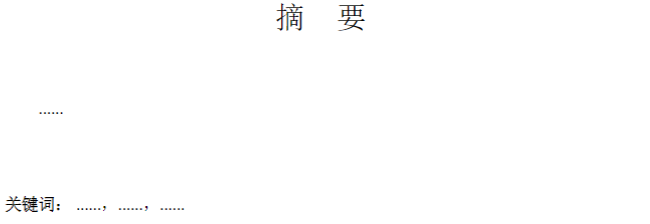
\includegraphics[width=0.45\textwidth]{1_1.png}}
      \subcaptionbox{......。}{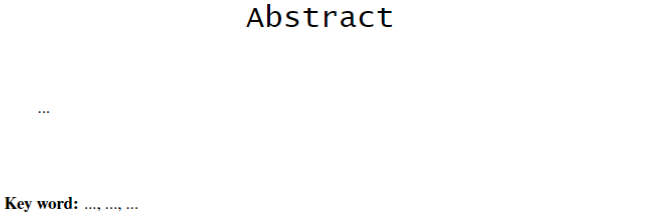
\includegraphics[width=0.45\textwidth]{1_2.png}}
      \caption{......。}\label{fig:图的标签}
\end{figure}

......

\section{国内外研究现状}

......

\section{研究挑战与目标}

......

\begin{enumerate}[wide=\parindent]
      \item ......
      \item ......
      \item ......
\end{enumerate}

......

\section{章节内容组织}

......


% % ChapterX.tex,论文的各个章节。

\chapter{22}

......

\section{第1节}

......

......公式~\ref{equ:公式}:
\begin{equation}\label{equ:公式}
    y=f(x), \quad x \in \symbb{R}^{n}, y \in \{0,1\},
\end{equation}
其中,......

......

\section{第2节}

......见图~\ref{fig:图像}。

\begin{figure}[!htbp]
    \centering
    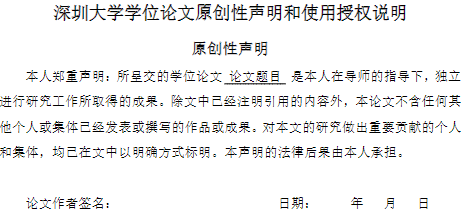
\includegraphics[width=0.7\textwidth]{2.png}
    \caption{......。
    }\label{fig:图像}
\end{figure}

......

\section{第3节}

......

......请见表~\ref{tab:表格}。

\begin{table}[!htbp]
    \caption{......。}\label{tab:表格}
    \centering
    \footnotesize
    \setlength{\tabcolsep}{4pt}{
        \begin{tabular}{ccc}
            \hline
            c1    & c2  & c3        \\ \hline
            r1    & 111 & 2333      \\
            r2    & 666 & 12580     \\ \hline
        \end{tabular}}
\end{table}

......

\section{本章小结}

......


% % ChapterX.tex,论文的各个章节。

\chapter{333}

......

\section{第1节}

......

\subsection{第1.1节}

......

\subsection{第1.2节}

......

\subsection{第1.3节}

......

\section{第2节}

......

\section{第3节}

......

\section{本章小结}

......


% % ChapterX.tex,论文的各个章节。

\chapter{4444}

......

\section{第1节}

......

\section{第2节}

......

\section{第3节}

......

\section{本章小结}

......


% % 结论

\chapter[结论]{结\quad{}论}

\section{研究总结}

......

\section{主要贡献与创新}

......

\section{不足与展望}

......


\backmatter  % 初始化其他部分环境,不建议注释

\szubibliography  % 导入参考文献

% % 附录

\chapter[附录]{附\quad{}录}

\section*{附录1:......}

......
  % 导入附录

% % 添加答辩记录
% 建议分三个独立的PDF或图像。\szuaddpdf包含两个参数,[]中为可选参数,用于生成目录,{}中为文件名,默认在Image下
% \szuaddpdf[指导教师对研究生学位论文的学术评语]{pingyu.pdf}
% \szuaddpdf[学位论文答辩委员会决议书]{dabian1.pdf}
% \szuaddpdf{dabian2.pdf}  % 前一页生成目录即可

% % 致谢

\chapter[致谢]{致\qquad{}谢}

......
  % 导入致谢  % 盲审版,注释掉此处

% % 研究成果

\chapter{攻读硕士学位期间的研究成果}

%% 可直接使用引用的格式
\begin{enumerate}[label = {[\arabic*]}]
    \item Cormen T H, Leiserson C E, Rivest R L, et al. Introduction to algorithms[M]. MIT press, 2022.
    \item LeCun Y, Bengio Y, Hinton G. Deep learning[J]. nature, 2015, 521(7553): 436-444.
    \item 李晓磊, 邵之江, 钱积新. 一种基于动物自治体的寻优模式: 鱼群算法[J]. 系统工程理论与实践, 2002, 22(11): 32-38.
\end{enumerate}

%% 或者区分开论文和专利
% \section*{论文}
% \begin{enumerate}[label = {[\arabic*]}]
%     \item Cormen T H, Leiserson C E, Rivest R L, et al. Introduction to algorithms[M]. MIT press, 2022.
%     \item LeCun Y, Bengio Y, Hinton G. Deep learning[J]. nature, 2015, 521(7553): 436-444.
% \end{enumerate}
% \section*{专利}
% \begin{enumerate}[label = {[\arabic*]}]
%     \item 李晓磊, 邵之江, 钱积新. 一种基于动物自治体的寻优模式: 鱼群算法[J]. 系统工程理论与实践, 2002, 22(11): 32-38.
% \end{enumerate}
  % 导入研究成果  % 盲审版,注释掉此处

\end{document}

% 查重时,PaperYY等网站会把封面、原创性申明、附录、致谢等算进去。将摘要-参考文献部分的PDF拆分出来,再进行PaperYY等网站的查重。
% 若是使用PaperYY查重,可使用https://www.ilovepdf.com/zh-cn/split_pdf网页或者其他PDF拆分工具。
